% !TeX encoding = UTF-8
% !TeX spellcheck = fr_FR
\documentclass[french,12pt,a4paper,titlepage,openright,openbib]{report}

\usepackage[utf8]{inputenc}
\usepackage[T1]{fontenc}
\usepackage[french]{babel}
\usepackage[default]{gillius}

\usepackage{graphicx}
\usepackage{lipsum}
\usepackage{array, caption, tabularx,  ragged2e,  booktabs}
\usepackage[pdfborder={0 0 0}]{hyperref}
\usepackage[xindy,toc]{glossaries}
\usepackage{titlesec}
\usepackage{color}
\usepackage{blindtext}
\usepackage{fancyhdr}
\usepackage{lastpage}
\usepackage[pages=some]{background}
\usepackage[pass]{geometry}
\usepackage{afterpage}
\usepackage{emptypage}
\usepackage{fancybox}
\usepackage{multicol}


% !TeX encoding = UTF-8
% !TeX spellcheck = fr_FR
% !TeX root = RapportMi3A.tex

%defini le style de couverture
\fancypagestyle{couverture}{
	\fancyhf{}
	\renewcommand \headrulewidth{0pt}
	\renewcommand \footrulewidth{0pt}
}

%default header & footer
\fancyhf{}
%redefinition du footer
\fancyfoot[C]{Page \textbf{\thepage} sur \textbf{\pageref{LastPage}}}
\renewcommand \footrulewidth{0pt}

%definition du header
\fancyhead[L]{\raisebox{-0.2 \height}{\includegraphics[width=2cm]{logo_nxp}}}
\fancyhead[R]{\textsc Rapport de mi-parcours 3A}
\renewcommand \headrulewidth{0pt}

%colors
\definecolor{gray75}{gray}{0.75}
\definecolor{aqua}{RGB}{0,164,167}
\definecolor{petrol}{RGB}{0,112,136}

\definecolor{nxpblue}{RGB}{123,177,219}
\definecolor{nxporange}{RGB}{249,181,0}
\definecolor{nxpgreen}{RGB}{201,210,0}

\parindent=0in
\parskip=8pt

%margins 1 inch
\addtolength{\oddsidemargin}{-.5in}
\addtolength{\evensidemargin}{-.5in}
\addtolength{\textwidth}{1.2in}

\addtolength{\topmargin}{-.5in}
\addtolength{\textheight}{0.8in}

%ajoute une page blanche
\newcommand{\blankpage}{%
	\null
	\thispagestyle{empty}%
	\addtocounter{page}{-1}%
	\newpage}
%ajouter un hespace de 20pt
\newcommand{\hsp}{\hspace{20pt}}
%numérotaiton romaine
\renewcommand\thechapter{\Roman{chapter}}
\renewcommand\thesection{\Roman{section}}
\renewcommand \thesubsection {\thesection.\Roman{subsection}}

%modification du style de chapitre
\titleformat{\chapter}[hang]{\Huge\bfseries}{\thechapter\hsp\textcolor{gray75}{|}\hsp}{0pt}{\Huge\bfseries}
\titlespacing{\chapter}{0pt}{0pt}{12pt}

%Renomme Bibliogrphy en
%\renewcommand{\bibname}{Références}

%redefini le style plain qui est utilisé sur les premières pages de chapitre
\fancypagestyle{plain}{%
	\fancyhf{} % clear all header and footer fields
	\fancyfoot[C]{Page \textbf{\thepage} sur \textbf{\pageref{LastPage}}} % except the center
	\fancyhead[L]{\raisebox{-0.2 \height}{\includegraphics[width=2cm]{logo_nxp}}}
	\fancyhead[R]{\textsc Rapport de mi-parcours 3A}
	\renewcommand \headrulewidth{0pt}
	\renewcommand{\footrulewidth}{0pt}}



\graphicspath{{template/}{img/}}

\title{Rapport final de troisième année}
\author{Jennifer Gr\"{a}nicher}
\date{11 juin 2018}

\pagestyle{fancy}


\makeglossaries
\newglossaryentry{mifare}
{
	name=MIFARE,
	description={Marque de NXP incluant une large gamme de circuits intégrés sans contact},
}
\newglossaryentry{desfire}
{
	name=DESFire,
	description={Marque de la famille MIFARE qui permet de créer des systèmes de cartes sécurisées grâce à l'alliance de la cryptographie et du sans contact},
}
\newglossaryentry{mooc}
{
	name=MOOC,
	description={Massive Open Online Course, formation ou cours en ligne},
	plural=MOOCs
}
\newacronym{nfc}{NFC}{Near Field Communication}
\newacronym{jee}{JEE}{Java Entreprise Edition}

\begin{document}
% !TeX encoding = UTF-8
% !TeX spellcheck = fr_FR
% !TeX root = RapportMi3A.tex

\backgroundsetup{
	scale=1,
	color=black,
	opacity=1.0,
	angle=0,
	contents={%
		\includegraphics[width=\paperwidth, height=\paperheight]{cover_tmpl}
	}%
}

{
	\BgThispage
	\thispagestyle{couverture}
	
	\newgeometry{headheight=80pt, top=6cm, headsep=3cm}
	
	\makeatletter
	{\LARGE\bfseries\@title\par}
	{\color{aqua}Informatique par apprentissage \\
	\color{aqua}Année universitaire 2017-2018}
	\hfill
	\vspace{0.5cm}
	
	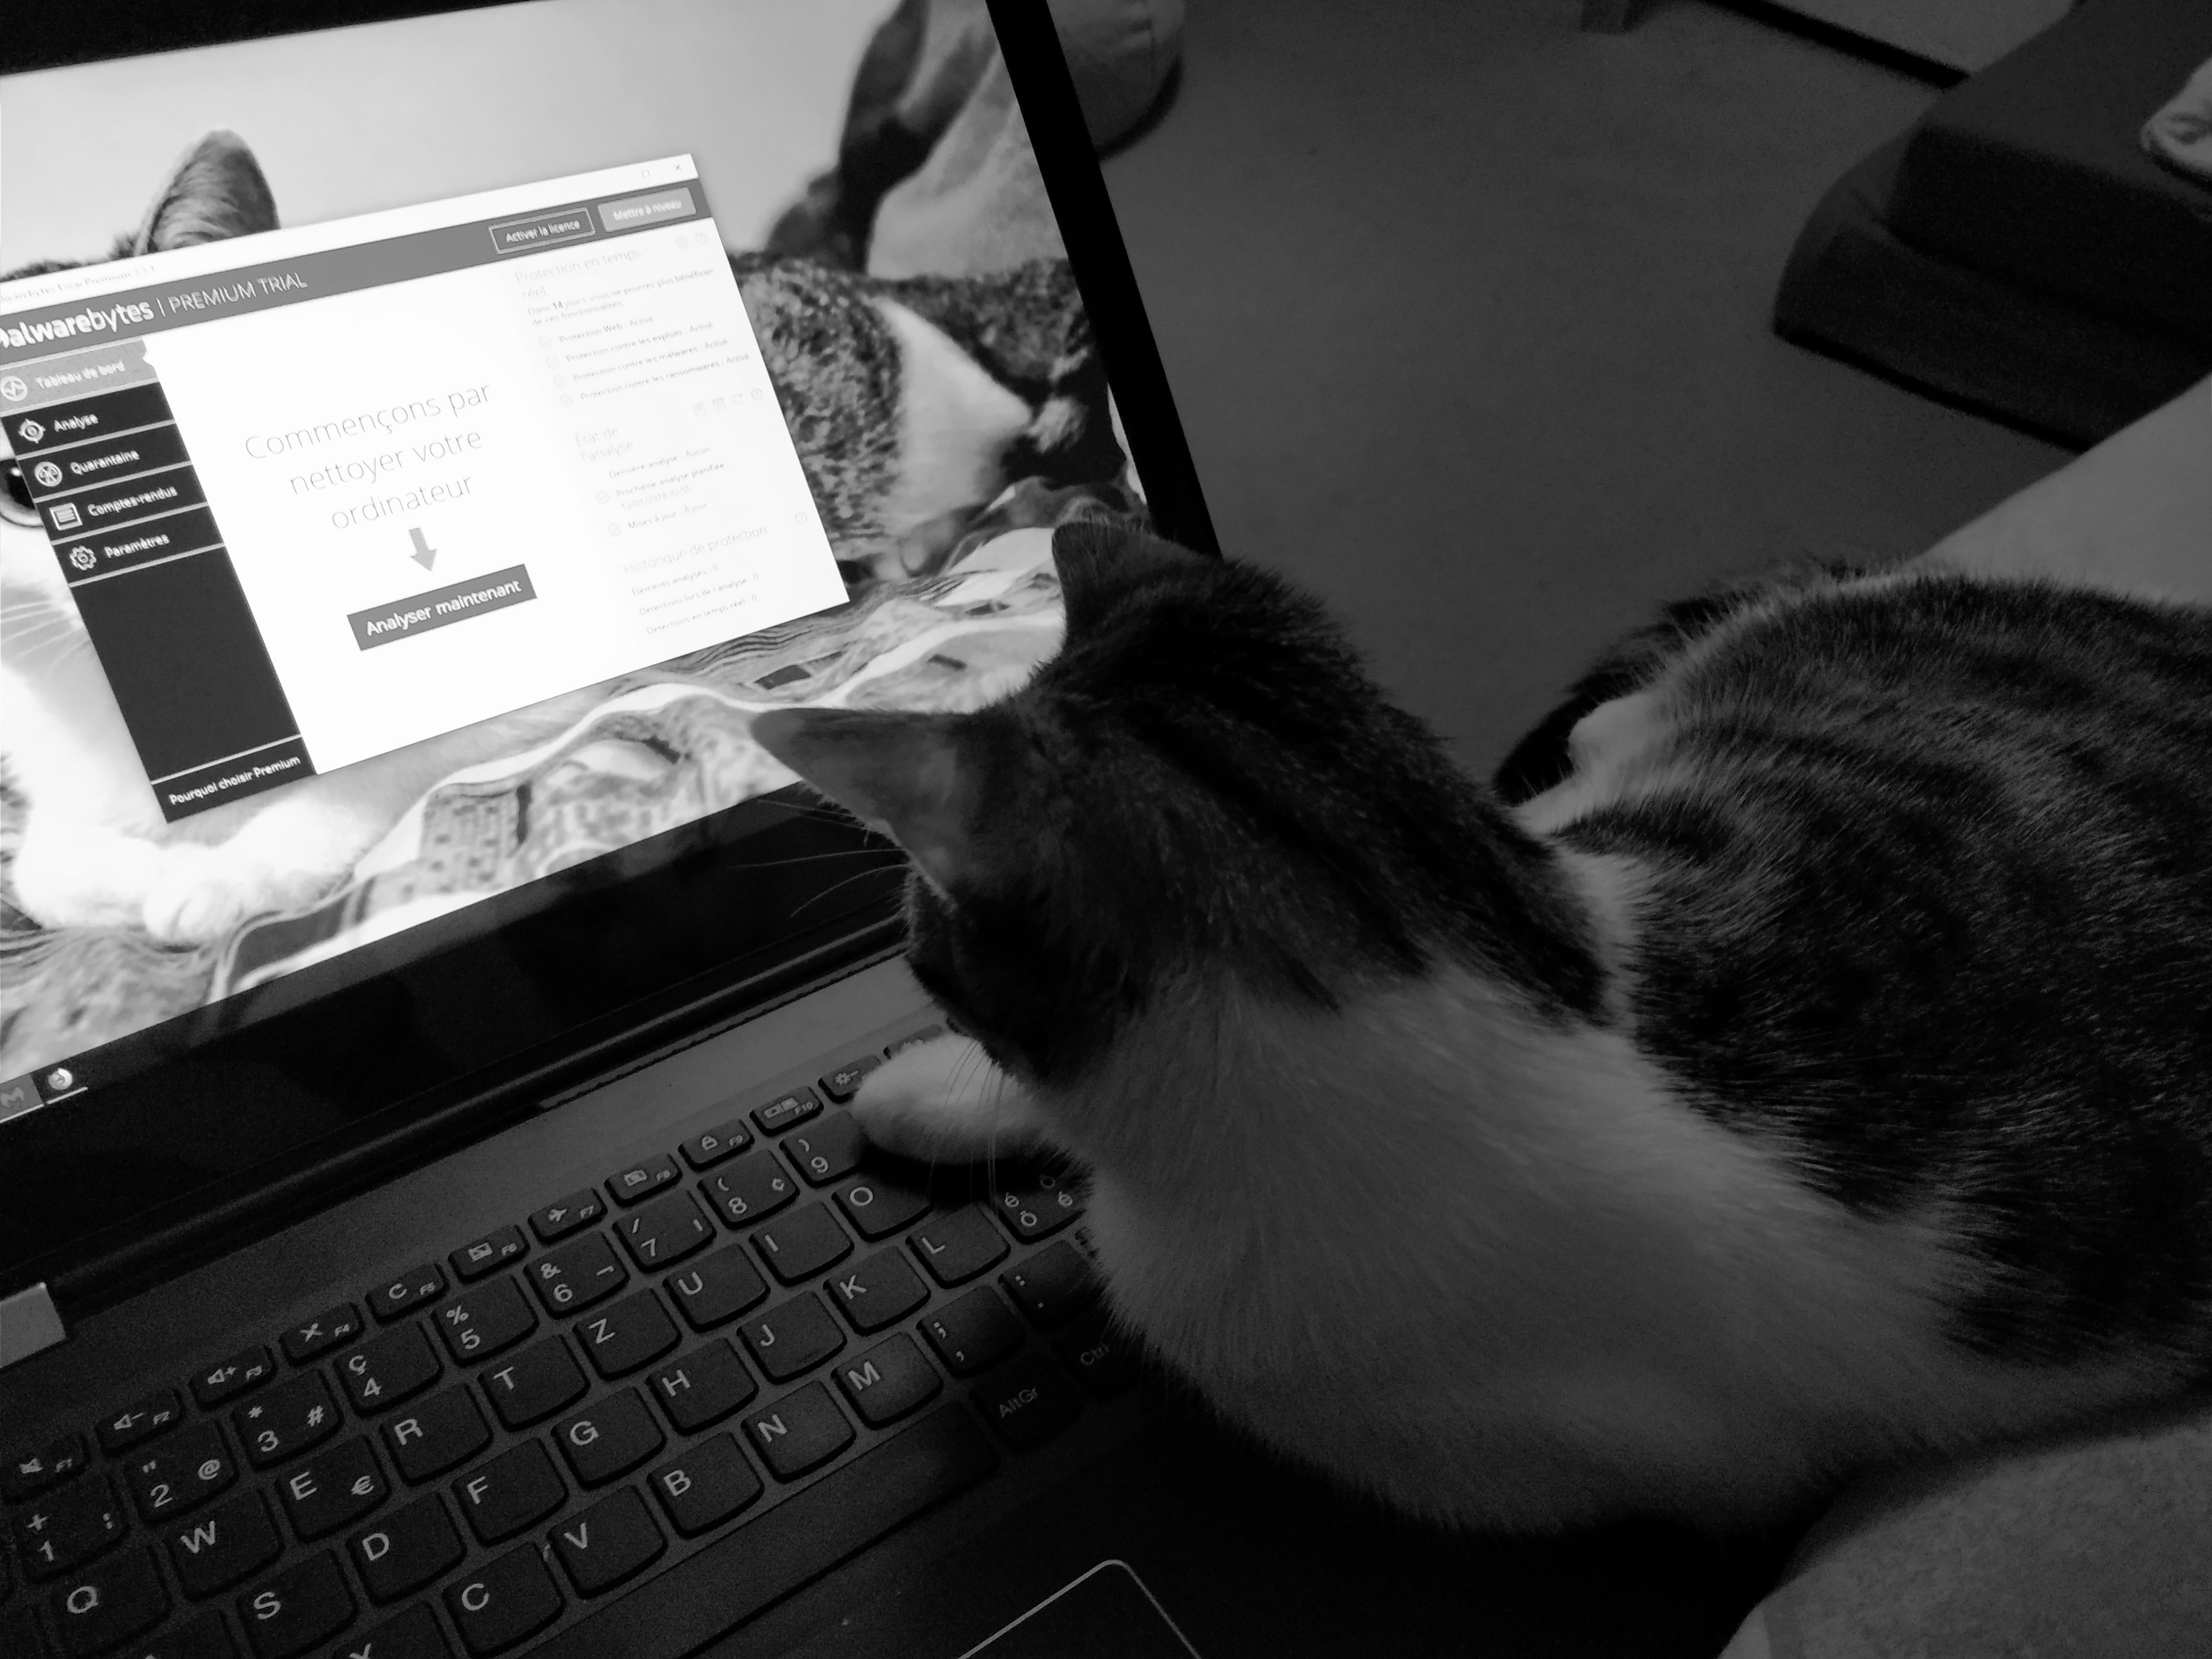
\includegraphics[width=15cm]{scylla}
	\vspace{0.5cm}
	
	\begin{minipage}[c]{0.5\textwidth}
	Tuteur école \par
	{\color{aqua} Wilfried \bsc{Aubry}}
	
	\vspace{0.5cm}
	
	Maître d'apprentissage \par
	{\color{aqua} Nicolas \bsc{Guillerm}}
	\end{minipage}
	\begin{minipage}[c]{0.5\textwidth}
	Auteur \par
	{\color{aqua} Jennifer \bsc{Gränicher}}
	
	\vspace{0.5cm}
	
	Date \par
	{\color{aqua} \@date}
	\end{minipage}
	
		
		
	
	\makeatother
	
	\vfill
	
	\afterpage{\blankpage}
	\restoregeometry
}


\maketitle

\chapter*{Remerciements}
J'aimerais remercier toutes les personnes qui ont contribué au bon déroulement de ces trois dernières années d'apprentissage, au sein de l'entreprise NXP Semiconductors, et au sein de l'ENSICAEN.

Je tiens particulièrement à remercier Virginie Jobard qui m'a épaulée et aidée à prendre mes repères au début.

Je souhaiterais également remercier Didier Graignic qui a su prendre le relais et m'aiguiller au cours de ma mission sur le projet MOOCTab \cite{website:mooctab} \cite{website:mooctabitea}.

J'aimerais aussi remercier Nicolas Guillerm pour toute l'aide qu'il a apporté que ce soit pour le rapport ou les missions au sein de l'entreprise.

Je remercie également Wilfried Aubry qui a été de bon conseil et qui a su apporter une grande aide.

Je tiens également à remercier mes collègues chez NXP pour leur aide et leur soutien.

\tableofcontents

\chapter*{Historique}
\begin{table}[ht]
	\label{tab:historique}
	\centering
	\begin{tabular}{|c|c|c|c|}
		\hline
		{\bf Version} & {\bf Date} & {\bf Rédigé par}    & {\bf Mise à jour}    \\
		\hline
		2.0           & 28/05/2018 & Jennifer Gränicher  & Édition du document \\
		\hline
		2.1           & 05/06/2018 & Jennifer Gränicher  & Mise en page \\
		\hline
		2.2           & 11/06/2018 & Jennifer Gränicher  & Finalisation \\
		\hline
	\end{tabular}
\end{table}

\vspace{2cm}

{\let \clearpage \relax \chapter*{Diffusion}}
\begin{table}[ht]
	\label{tab:diffusion}
	\centering
	\begin{tabular}{|c|c|c|c|}
		\hline
		{\bf Destinataire} & {\bf Société}      & {\bf Fonction}   		 & {\bf Date}\\
		\hline
		Nicolas Guillerm   & NXP Semiconductors & Maitre d'apprentissage & 07/06/2018 \\
		\hline
		Wifried Aubry      & ENSICAEN 			& Tuteur				 & 11/06/2018 \\
		\hline
	\end{tabular}
\end{table}

\chapter{Introduction}
Ce document parle de mes trois années d'apprentissage au sein de NXP Semiconductors, de Septembre 2015 à Juin 2018.

Une première partie concerne l'environnement au sein duquel j'ai progressé durant ces trois ans.
Une seconde partie traite des projets passés et en cours et leurs impacts sur mon évolution professionnelle.

\chapter{Environnement de travail}
NXP Semiconductors est une société fabricant des semi-conducteurs.
L'entreprise possède plusieurs sites répartis dans plus de 33 pays dont 4 en France, le tout totalisant 31'000 employé\textperiodcentered e\textperiodcentered s.

NXP est actuellement leader mondial dans plusieurs domaines tels que:

\begin{itemize}
\item L'identification (e-passeport, transport, accès, ...);
\item L'automobile;
\item Les microcontrôleurs à usages généraux;
\item ...
\end{itemize}

%insérer ici les coeurs de métier
\section{NXP Caen}

L'équipe avec laquelle je travaille est aujourd'hui composée de Nicolas Guillerm, Dominique Défossez et moi-même. Dominique Défossez est responsable stratégie et partenariat pour NXP Semiconductors en France, il s'occupe notamment du management des projets européens.
Cette équipe travaille pour le compte de NXP sur le projet MOOCTab qui se clôturera à la fin du mois de juin.
%%%%%%%%%%%%%%

\section{Actualités Qualcomm}
En octobre 2016 Qualcomm annonçait son souhait de racheter NXP Semiconductors. La commission américaine avait approuvé ce rachat mais la commission européenne avait été saisie par une entreprise concurrente.

Après une enquête approfondie, la commission européenne a finalement accepté le rachat sous certaines conditions.

Le rachat a cependant été bloqué par la Chine qui avait mis son processus décisionnel en pause. Actuellement la Chine a annoncé une prise de décision proche, nous saurons donc dans les semaines à venir si le rachat est approuvé ou non.
%China approval



\chapter{Évolution au cours des projets}

Au cours de ma formation j'ai été amenée à travailler sur des petites tâches ponctuelles, principalement le développement d'applications Android. Ces applications avaient pour but de montrer différents usages de la technologie \gls{nfc}.
En deuxième année mes tâches ont progressivement évolué vers le projet européen MOOCTab qui occupait jusqu'à récemment la plus grande partie de mon temps.
En complément du projet MOOCTab j'ai commencé à travailler sur un projet qui met en scène l'utilisation de l'élément sécurisé comme lecteur.
En parallèle je suis consultée pour le projet d'Open Escape Book ainsi que la maintenance de l'application Labtab.

\section{Smartcampus}

Lors de mes débuts chez NXP il était clair que j'allais travailler principalement sur des applications promouvant la \gls{nfc}. Comme je m'y attendais j'ai donc travaillé sur du WEB et du mobile (Android).
Si au début j'ai travaillé sur des technologies avec lesquelles j'étais déjà à l'aise, j'ai progressivement évolué vers des langages que je connaissais moins et vers des tâches qui ne relevaient pas exclusivement du développement logiciel.

C'est avec le projet Smartcampus que j'ai commencé mon ascension. Ce projet était un concept de gestion de campus connectés(cf. : rapport 1A) dont le développement avait été commencé par d'autres apprentis avant moi. J'étais alors encore une technicienne lorsque j'ai débuté sur ce projet avec la création d'une interface WEB dans le cadre d'un stage précédant l'apprentissage.
La tâche de maintenance et migration qui m'avait ensuite été confiée relevait toujours de mes compétences techniques et me permettait de rester dans ma zone de confort tout en renforçant mes compétences techniques.

C'est dans le cadre du Smartcampus que m'avait été confié le développement d'une application de report d'incident (Incident Reporting). Ce projet m'a permis d'assoir mes compétences techniques tout en acquérant de nouvelles mais aussi et surtout d'appliquer des méthodes de gestion de projet. C'est la première mission qui m'a permis de dialoguer avec des employé\textperiodcentered e\textperiodcentered s d'autres services. Au travers du développement du report d'incident j'ai pu apprendre à collecter les besoins utilisateur\textperiodcentered rice\textperiodcentered s et les exprimer, c'était aussi un premier pas vers plus d'autonomie.

Le projet Labtab fait partie du projet Smartcampus tout en étant une partie séparée puisqu'il est utilisé en interne pour la gestion des emprunts matériel. C'est un projet sur lequel j'ai surtout effectué la mise en place et maintenance au niveau de la disponibilité du serveur.
J'ai eu l'occasion d'effectuer un support anecdotique au niveau de l'application Android. Enfin récemment il m'a été demandé d'apporter quelques modifications pour ajouter des fonctionnalités sur l'interface WEB. Néanmoins ces petites modifications m'ont appris à être à l'écoute des besoins clients qui ne sont pas toujours les mêmes 

En terme de serveur je me suis heurtée à des problèmes administratifs internes suite auxquels j'ai du envisager d'autres solutions pour l'utilisateur principal de cette application. De plus il a fallut que je trouve une solution qui permette de maintenir le fonctionnement de cette application suite à mon départ à la fin de mon contrat. 

Cela m'a permis de me rendre compte des problèmes qui peuvent être rencontrés au quotidien sur le déploiement d'une solution ainsi que la nécessité d'avoir un support, sans quoi une application ne peut survivre.


\section{MOOCTab}

Le projet MOOCTab a, pour moi, été l'expérience la plus complète que j'aie pu  vivre au cours de ces trois années. En effet je suis arrivée sur le projet en cours de route, il m'a été demandé de réaliser plusieurs démonstrateurs qui avaient des objectifs très différents et qui requérait des compétences très différentes et que je ne maîtrisais pas toujours.

La plus grosse difficulté a été pour moi d'aller me renseigner auprès de mes collègues compétents dans les domaines que je ne connaissais pas, je manquais alors de confiance en moi et était un peu intimidée dans un environnement nouveau pour moi. Heureusement cela a été l'occasion pour moi de gagner en confiance et en technicité.

De plus alors que je commençais à prendre confiance il a fallu faire face à 2 changements consécutifs de maître d'apprentissage à quelques mois d'écart. Si au début cela était difficile et confus cela m'a permis de gagner en autonomie mais aussi en confiance car cela m'a fait prendre des initiatives. J'ai du apprendre à gérer ces petites crises puisqu'il a fallu redéfinir les tâches que j'allais devoir effectuer. Par exemple il était initialement prévu que Didier Graignic s'occupe entièrement de la partie concernant le câblage matériel, dont j'ai finalement hérité à son départ.

 


\chapter{Bilan}

\chapter{Conclusion}

\printglossary[title={Glossaire}]

\bibliography{mybib}{}
\bibliographystyle{plain}
	
\end{document}


